\section{Dữ liệu và tiền xử lý}
\label{sec:du_lieu}

Quy trình tiền xử lý chuyển ảnh gốc thành vectơ HOG. Nhóm lưu kết quả trung gian của từng bước để các mô hình có thể sử dụng lại cùng dữ liệu và cách chia tập.

\subsection{Phân tích khám phá dữ liệu}

\subsubsection*{Quy mô và phân bố lớp}

Bộ dữ liệu gốc có 9.544 ảnh định dạng JPEG, chia thành sáu lớp. Bảng~\ref{tab:dataset_stats} tóm tắt số ảnh và kích thước ảnh của từng lớp.

\begin{table}[H]
\centering
\caption{Thống kê bộ dữ liệu SOHAS gốc theo lớp}
\label{tab:dataset_stats}
\small
\begin{tabularx}{\linewidth}{@{}lXrrcc@{}}
\toprule
\textbf{Lớp} & \textbf{Ý nghĩa} & \textbf{Số ảnh} & \textbf{Tỷ lệ} &
\shortstack{\textbf{Rộng $\times$ cao}\\\textbf{(trung vị)}} &
\shortstack{\textbf{Tỷ lệ khung}\\\textbf{(trung vị)}} \\
\midrule
\texttt{pistol}     & Súng ngắn       & 3.975 & 41,6\% & 156 $\times$ 124 & 1,34 \\
\texttt{knife}      & Dao             & 2.349 & 24,6\% & 156 $\times$ 148 & 1,17 \\
\texttt{smartphone} & Điện thoại      & 1.184 & 12,4\% & 397 $\times$ 559 & 0,73 \\
\texttt{monedero}   & Ví              &   813 &  8,5\% & 258 $\times$ 231 & 1,15 \\
\texttt{billete}    & Tiền giấy       &   777 &  8,1\% & 254 $\times$ 216 & 1,21 \\
\texttt{tarjeta}    & Thẻ ngân hàng   &   446 &  4,7\% & 186 $\times$ 145 & 1,38 \\
\midrule
\textbf{Tổng}       &                 & \textbf{9.544} & 100\% & 182 $\times$ 164 & 1,25 \\
\bottomrule
\end{tabularx}
\end{table}

Phân bố lớp, kích thước ảnh và tỷ lệ khung ảnh là ba đặc điểm ảnh hưởng đến cách nhóm xử lý và đánh giá dữ liệu.

\begin{itemize}
  \item \textbf{Số ảnh chênh lệch lớn giữa các lớp.} Lớp \texttt{pistol} có 3.975 ảnh, gấp 8,9 lần lớp \texttt{tarjeta} (446 ảnh). Một bộ phân loại luôn dự đoán lớp súng ngắn đạt độ chính xác 41,6\% trên bộ dữ liệu gốc. Vì vậy, nhóm dùng trọng số lớp cân bằng khi huấn luyện và chọn macro-F1 làm chỉ số chính (Mục~\ref{sec:metrics}).
  \item \textbf{Ảnh súng ngắn và dao thường nhỏ hơn ảnh điện thoại.} Chiều rộng trung vị của ảnh súng ngắn và dao là 156 điểm ảnh, so với 397 điểm ảnh ở lớp điện thoại. Sau khi làm sạch, 52\% số ảnh có cả hai chiều nhỏ hơn 224 điểm ảnh. Tỷ lệ này là 60\% ở lớp \texttt{pistol}, 62\% ở lớp \texttt{knife} và 23\% ở lớp \texttt{smartphone}. Mức chênh lệch này đặt ra câu hỏi liệu mô hình có sử dụng các dấu hiệu do phóng to ảnh tạo ra hay không.
  \item \textbf{Tỷ lệ khung ảnh thay đổi nhiều.} Tỷ số chiều rộng trên chiều cao dao động từ 0,05 đến 19,7. Có 18,6\% số ảnh có tỷ số lớn hơn 2 hoặc nhỏ hơn 0,5. Với những ảnh này, hai cách đưa ảnh về kích thước vuông có thể tạo ra vectơ HOG khác nhau đáng kể (Mục~\ref{sec:resize}).
\end{itemize}

\begin{figure}[H]
  \centering
  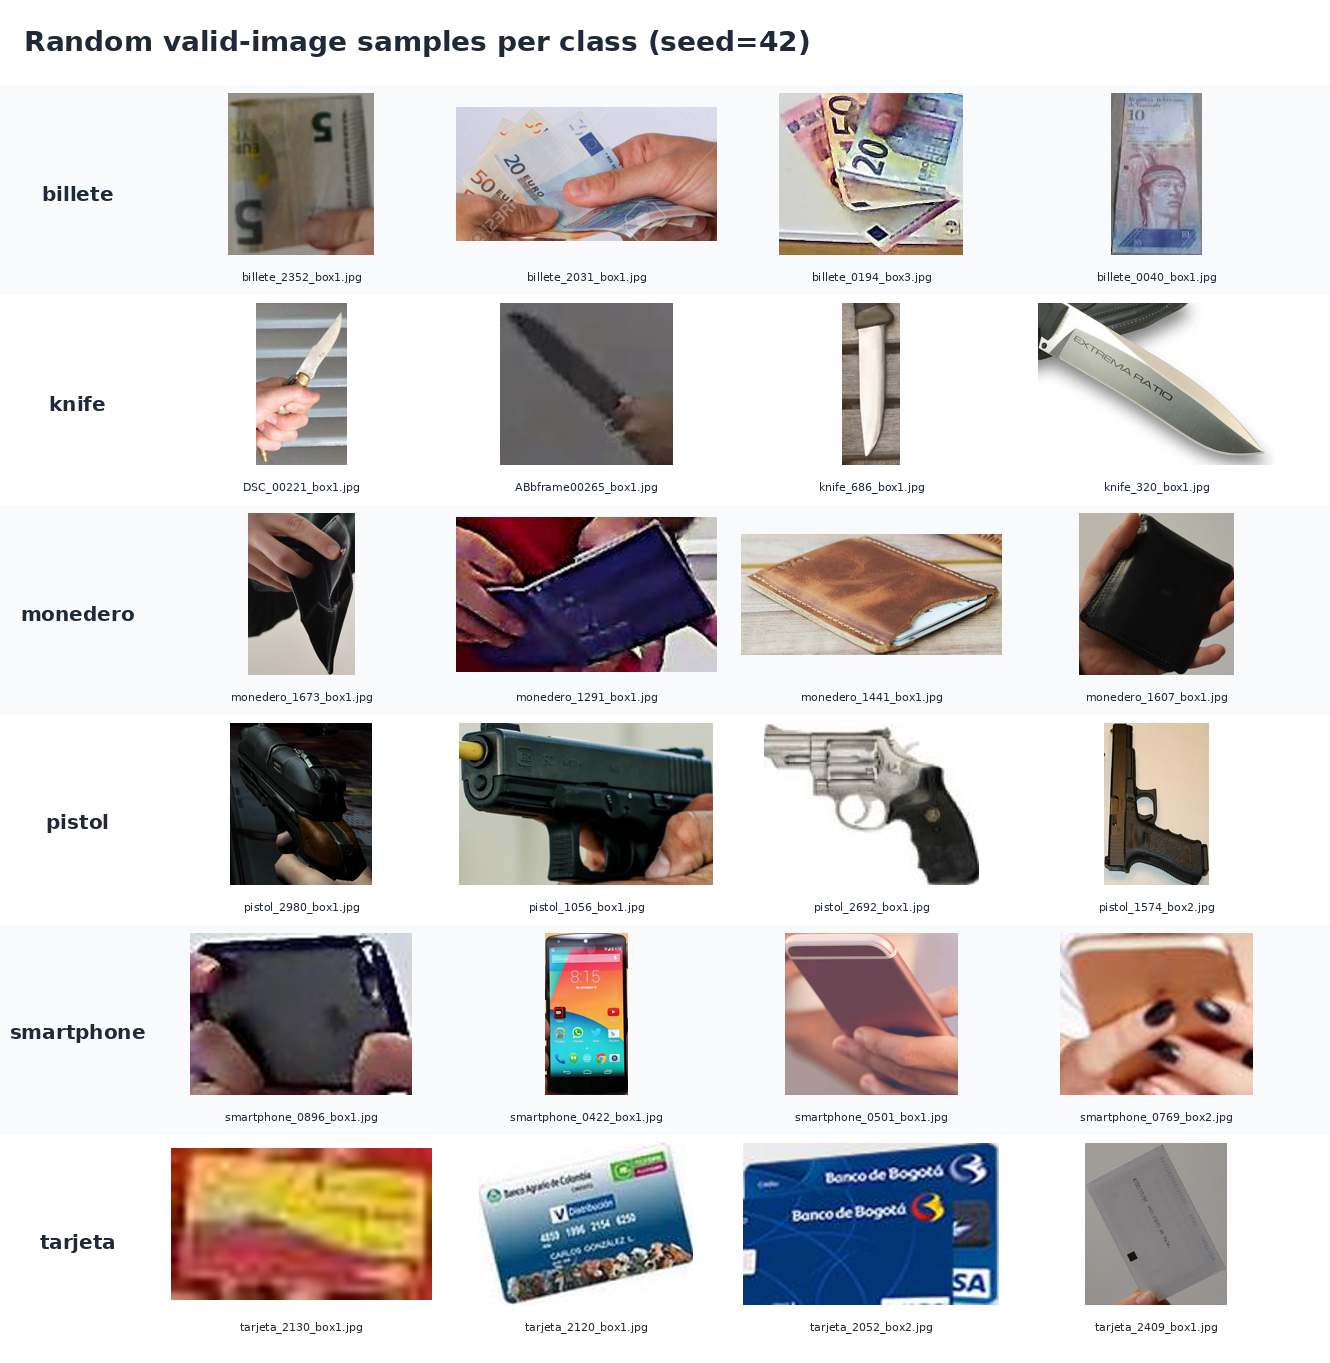
\includegraphics[width=0.85\textwidth]{sample_images.png}
  \caption{Bốn ảnh lấy ngẫu nhiên từ mỗi lớp. Một số vật thể bị bàn tay che khuất một phần.}
  \label{fig:samples}
\end{figure}

\subsubsection*{Đặc điểm hình ảnh}

Các ảnh trong SOHAS đã được cắt quanh vật thể. Trong các ví dụ ở Hình~\ref{fig:samples}, bàn tay xuất hiện ở cả sáu lớp và có thể che khuất một phần vật thể. Các cạnh và đường cong của bàn tay cũng góp phần vào vectơ HOG tính trên toàn ảnh.

\begin{figure}[H]
  \centering
  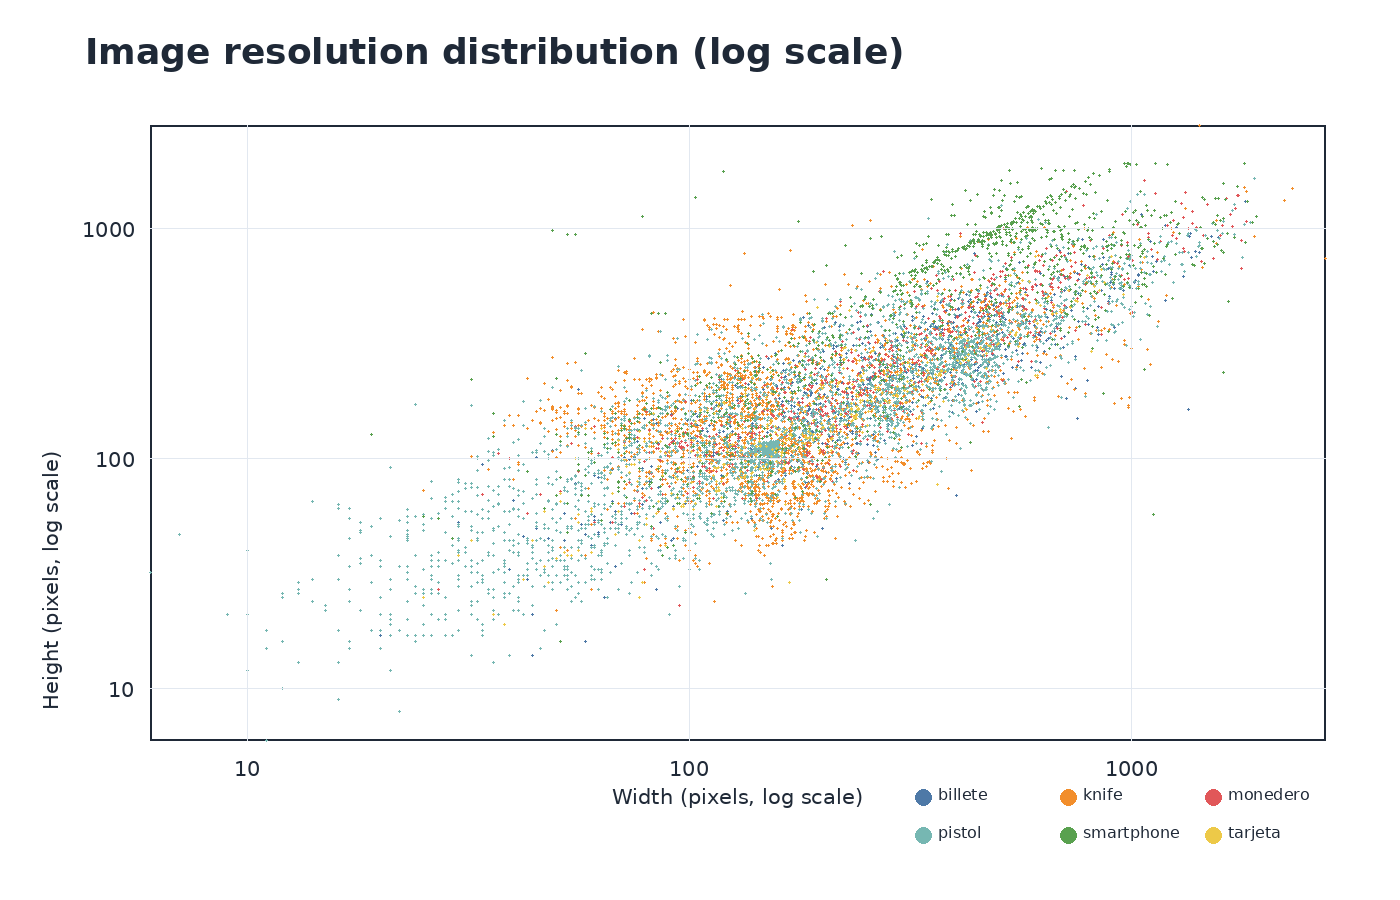
\includegraphics[width=0.85\textwidth]{image_resolution.png}
  \caption{Phân bố chiều rộng và chiều cao của ảnh theo thang logarit. Ảnh súng ngắn và dao tập trung ở vùng kích thước nhỏ hơn ảnh điện thoại.}
  \label{fig:resolution}
\end{figure}

\subsection{Quy trình tiền xử lý}

Hình~\ref{fig:pipeline} tóm tắt năm bước tiền xử lý, từ kiểm tra tệp ảnh đến trích xuất HOG.

\begin{figure}[H]
\centering
\small
\setlength{\fboxsep}{4pt}
\begin{tabular}{c}
\fbox{\parbox{0.8\textwidth}{\centering \textbf{1. Kiểm tra ảnh} -- giải mã từng ảnh, ghi lại kích thước và định dạng}} \\
$\downarrow$ \\
\fbox{\parbox{0.8\textwidth}{\centering \textbf{2. Loại ảnh trùng} -- so sánh mã băm SHA-256, giữ một bản đại diện cho mỗi nhóm ảnh trùng}} \\
$\downarrow$ \\
\fbox{\parbox{0.8\textwidth}{\centering \textbf{3. Chuẩn hóa kích thước} -- tạo ảnh 224 $\times$ 224 theo nhánh \emph{direct} và nhánh \emph{padding}}} \\
$\downarrow$ \\
\fbox{\parbox{0.8\textwidth}{\centering \textbf{4. Chia dữ liệu} -- tập train, tập validation và tập test theo tỷ lệ 4/1/1, có phân tầng theo lớp}} \\
$\downarrow$ \\
\fbox{\parbox{0.8\textwidth}{\centering \textbf{5. Trích xuất HOG} -- 26.244 đặc trưng cho mỗi ảnh}} \\
\end{tabular}
\caption{Các bước tiền xử lý dữ liệu}
\label{fig:pipeline}
\end{figure}

\subsubsection{Kiểm tra ảnh lỗi và loại ảnh trùng lặp}

Nhóm dùng Pillow để kiểm tra khả năng giải mã, đồng thời ghi nhận kích thước và định dạng của từng ảnh. Cả 9.544 ảnh đều giải mã thành công.

Nhóm tính mã băm SHA-256 trên nội dung của từng tệp để tìm các bản sao giống nhau. Kết quả có một cặp tệp trùng thuộc lớp \texttt{pistol}. Nhóm giữ một tệp đại diện, nên bộ dữ liệu sau khi làm sạch còn \textbf{9.543 ảnh}.

Loại bản sao trước khi chia dữ liệu giúp tránh trường hợp cùng một ảnh xuất hiện trong cả tập train và tập test. Bước này phát hiện các tệp trùng nội dung ở mức byte. Các ảnh gần trùng, chẳng hạn ảnh được mã hóa lại, có thể có mã băm khác nhau.

\begin{figure}[H]
  \centering
  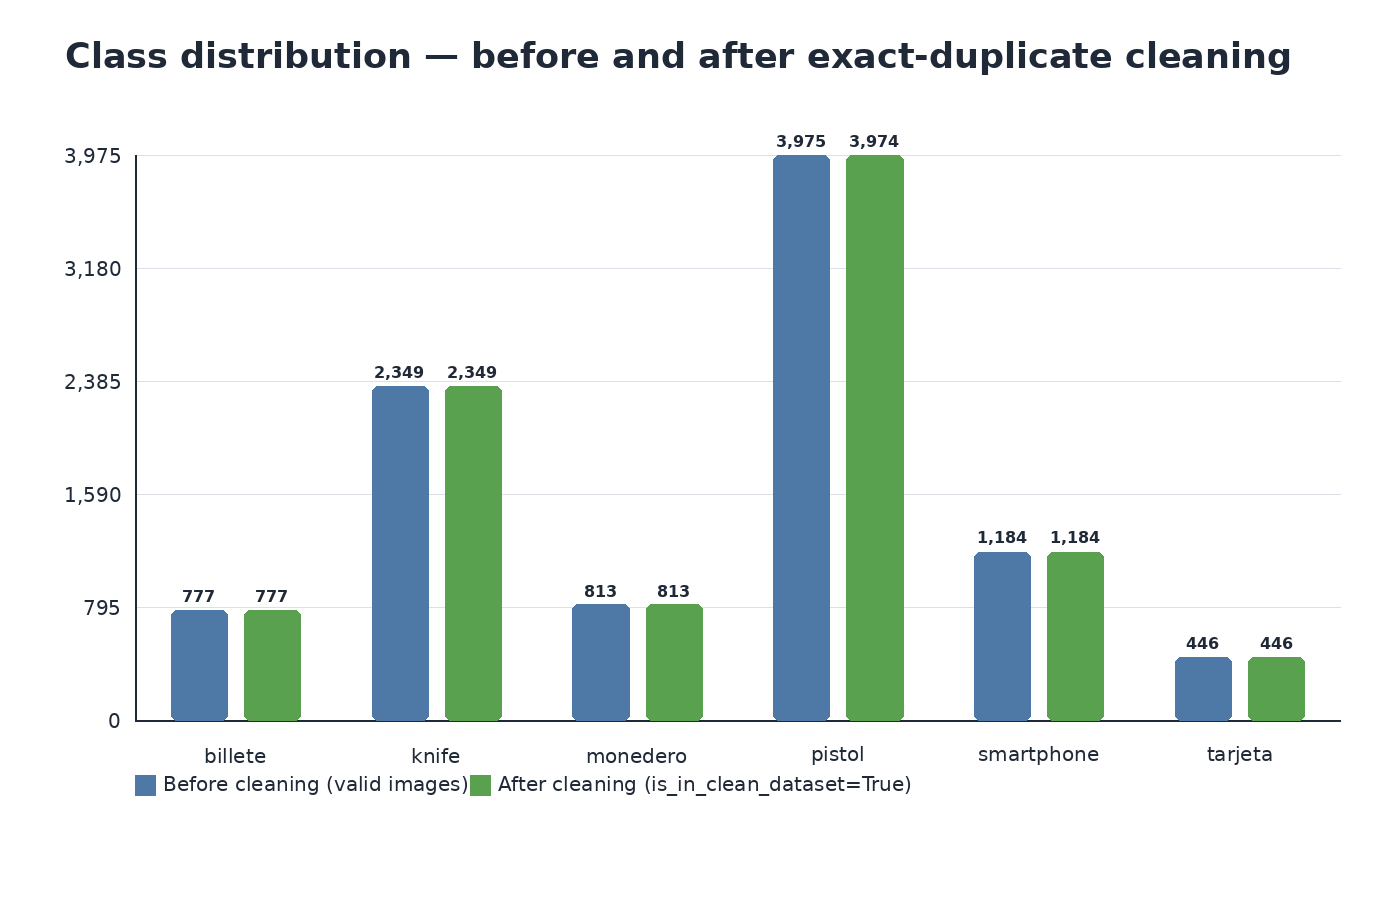
\includegraphics[width=0.8\textwidth]{class_distribution_before_after_cleaning.png}
  \caption{Phân bố lớp trước và sau khi làm sạch. Chỉ một ảnh của lớp \texttt{pistol} bị loại.}
  \label{fig:clean}
\end{figure}

\subsubsection{Chuẩn hóa kích thước theo hai nhánh}
\label{sec:resize}

Với cùng cấu hình ô và khối, các ảnh cần có cùng kích thước để vectơ HOG có cùng số chiều. Nhóm đưa ảnh về 224 $\times$ 224 điểm ảnh theo hai cách.

\begin{itemize}
  \item \textbf{Co giãn trực tiếp (\emph{direct}).} Nhóm đổi riêng chiều rộng và chiều cao về 224 điểm ảnh. Nếu ảnh ban đầu có dạng chữ nhật, hai chiều được co giãn theo các tỷ lệ khác nhau.
  \item \textbf{Giữ tỷ lệ và đệm viền (\emph{padding}).} Nhóm đổi kích thước theo cùng một hệ số trên hai chiều để cạnh dài bằng 224 điểm ảnh, rồi đệm phần còn lại bằng màu xám trung tính (giá trị 128 ở mỗi kênh).
\end{itemize}

Nhóm chọn màu xám trung tính để hạn chế chênh lệch cường độ sáng tại ranh giới giữa nội dung ảnh và phần đệm. Tùy độ sáng của ảnh, ranh giới này vẫn có thể tạo ra gradient và ảnh hưởng đến đặc trưng HOG.

Hai cách xử lý có thể ảnh hưởng đến HOG theo các hướng khác nhau. Co giãn trực tiếp làm thay đổi tỷ lệ khung ảnh, còn đệm viền giữ tỷ lệ nhưng dành một phần khung hình cho nền xám. Mục~\ref{sec:discussion} thảo luận kết quả so sánh.

\begin{lstlisting}[caption={Hàm tạo ảnh giữ tỷ lệ có đệm viền xám (rút gọn)},label={lst:padding}]
GRAY_BGR = (128, 128, 128)

def padded(image, target=224):
    h, w = image.shape[:2]
    scale = min(target / w, target / h)          # keep aspect ratio
    nw, nh = round(w * scale), round(h * scale)
    method = cv2.INTER_CUBIC if (w < target and h < target) else cv2.INTER_AREA
    resized = cv2.resize(image, (nw, nh), interpolation=method)
    left, top = (target - nw) // 2, (target - nh) // 2
    right, bottom = target - nw - left, target - nh - top
    return cv2.copyMakeBorder(resized, top, bottom, left, right,
                              cv2.BORDER_CONSTANT, value=GRAY_BGR)
\end{lstlisting}

\subsubsection{Lựa chọn phép nội suy}

Khi cả hai chiều của ảnh nhỏ hơn 224 điểm ảnh, nhóm dùng nội suy song khối (bicubic). Phép nội suy này xét một vùng lân cận lớn hơn nội suy song tuyến tính (bilinear), nên có thể cho chuyển tiếp khác tại các cạnh mà HOG ghi nhận.

Trong các trường hợp còn lại, chương trình dùng nội suy theo diện tích (area interpolation). Khi thu nhỏ ảnh, phép nội suy này tổng hợp thông tin từ vùng điểm ảnh tương ứng và có thể giảm hiện tượng răng cưa (aliasing).

\subsubsection{Chia dữ liệu}

Nhóm chia 9.543 ảnh thành tập train, tập validation và tập test theo tỷ lệ xấp xỉ 4/1/1.

\begin{itemize}
  \item \textbf{Phân tầng theo lớp (stratified splitting).} Nhóm áp dụng tỷ lệ chia cho từng lớp để phân bố lớp ở ba tập gần với phân bố của bộ dữ liệu sau khi làm sạch.
  \item \textbf{Chia theo nhóm.} Nếu dữ liệu có thông tin về nhóm ảnh trùng, chương trình xếp các ảnh cùng nhóm vào cùng một tập. Trong bộ dữ liệu đã làm sạch, mỗi nhóm trùng khớp theo SHA-256 chỉ còn một ảnh đại diện.
\end{itemize}

Chương trình sử dụng giá trị khởi tạo ngẫu nhiên (\emph{seed}) bằng 42. Bảng~\ref{tab:split} trình bày số ảnh của từng lớp trong mỗi tập.

\begin{table}[H]
\centering
\caption{Số ảnh của từng lớp trong ba tập dữ liệu}
\label{tab:split}
\begin{tabular}{@{}lrrrr@{}}
\toprule
\textbf{Lớp} & \textbf{Train} & \textbf{Validation} & \textbf{Test} & \textbf{Tổng} \\
\midrule
\texttt{pistol}     & 2.649 & 663 & 662 & 3.974 \\
\texttt{knife}      & 1.566 & 392 & 391 & 2.349 \\
\texttt{smartphone} &   789 & 198 & 197 & 1.184 \\
\texttt{monedero}   &   542 & 136 & 135 &   813 \\
\texttt{billete}    &   518 & 130 & 129 &   777 \\
\texttt{tarjeta}    &   297 &  75 &  74 &   446 \\
\midrule
\textbf{Tổng}       & \textbf{6.361} & \textbf{1.594} & \textbf{1.588} & \textbf{9.543} \\
\bottomrule
\end{tabular}
\end{table}

\subsubsection{Trích xuất đặc trưng HOG}

Nhóm chuyển ảnh sang ảnh xám rồi tính HOG~\cite{dalal2005hog}. HOG biểu diễn hướng và độ lớn của gradient cường độ sáng trong các vùng lân cận, qua đó mô tả cấu trúc cạnh của ảnh. Quy trình gồm bốn bước.

\begin{enumerate}
  \item \textbf{Tính gradient.} Từ đạo hàm theo hai trục $G_x$ và $G_y$, nhóm tính độ lớn $\sqrt{G_x^2 + G_y^2}$ và hướng $\operatorname{atan2}(G_y,G_x)$ của gradient. Gradient có độ lớn cao ở những vùng mà cường độ sáng thay đổi nhanh.
  \item \textbf{Lập biểu đồ hướng theo ô (cell).} Nhóm chia ảnh thành các ô 8 $\times$ 8 điểm ảnh và chia miền hướng $[0^\circ,180^\circ)$ thành chín khoảng. Hướng gradient được quy về miền này theo chu kỳ $180^\circ$. Mỗi điểm ảnh đóng góp vào biểu đồ theo độ lớn gradient của nó.
  \item \textbf{Chuẩn hóa theo khối (block).} Nhóm gộp 2 $\times$ 2 ô thành một khối và áp dụng L2-Hys lên vectơ của khối. Phương pháp này chuẩn hóa vectơ theo chuẩn L2, giới hạn các giá trị ở mức 0,2 rồi chuẩn hóa lại. Bước này giảm ảnh hưởng của chênh lệch độ tương phản giữa các vùng ảnh.
  \item \textbf{Ghép vectơ.} Các khối trượt chồng lên nhau với bước bằng một ô; vectơ của tất cả các khối được ghép thành vectơ đặc trưng của ảnh.
\end{enumerate}

Với ảnh 224 $\times$ 224 và ô 8 $\times$ 8, lưới có 28 $\times$ 28 ô và $27 \times 27 = 729$ khối. Mỗi khối có $2 \times 2 \times 9 = 36$ giá trị, nên vectơ của mỗi ảnh có số chiều
\[
  729 \times 36 = 26.244 \text{ đặc trưng}.
\]
Số đặc trưng lớn gấp hơn bốn lần số ảnh trong tập train (6.361). Chương~\ref{sec:thuc_nghiem} đánh giá dấu hiệu quá khớp bằng cách đối chiếu kết quả trên tập train và tập validation.

\begin{lstlisting}[caption={Cấu hình trích xuất HOG},label={lst:hog}]
from skimage.feature import hog

PARAMS = {"orientations": 9, "pixels_per_cell": (8, 8),
          "cells_per_block": (2, 2), "block_norm": "L2-Hys"}

gray = cv2.cvtColor(image, cv2.COLOR_BGR2GRAY)
features = hog(gray, **PARAMS).astype(np.float32)   # shape: (26244,)
\end{lstlisting}

\subsubsection{Chuẩn hóa đặc trưng và giảm chiều}

Nhóm đưa các đặc trưng có phương sai khác 0 về cùng thang đo trước khi huấn luyện. Nếu các đặc trưng có thang đo rất khác nhau, cùng một mức phạt lên hệ số mô hình có thể tác động khác nhau đến đóng góp của từng đặc trưng. Bộ chuẩn hóa chỉ học các hệ số biến đổi từ tập train rồi áp dụng chúng cho tập validation và tập test.

Với SVM RBF, nhóm dùng PCA để giảm vectơ đầu vào từ 26.244 xuống 256 chiều. Việc giảm chiều làm giảm số phép tính cho mỗi lần tính khoảng cách giữa hai vectơ. Nhóm dùng phương pháp PCA ngẫu nhiên (\emph{randomized PCA}) để ước lượng 256 thành phần chính từ tập train.

\subsubsection{Lưu trữ đặc trưng}

Nhóm lưu đặc trưng của mỗi nhánh trong một tệp NumPy \texttt{.npz}. Tệp chứa ma trận 9.543 $\times$ 26.244 kiểu số thực 32 bit, nhãn lớp, tập mà mỗi ảnh thuộc về, mã băm và cấu hình HOG. Nhờ đó, các lần huấn luyện có thể dùng lại vectơ HOG và cùng một cách chia dữ liệu.
